\section{Algorithm}
\label{section: Chapter4/algo}

\begin{figure}[h]
    \centering
    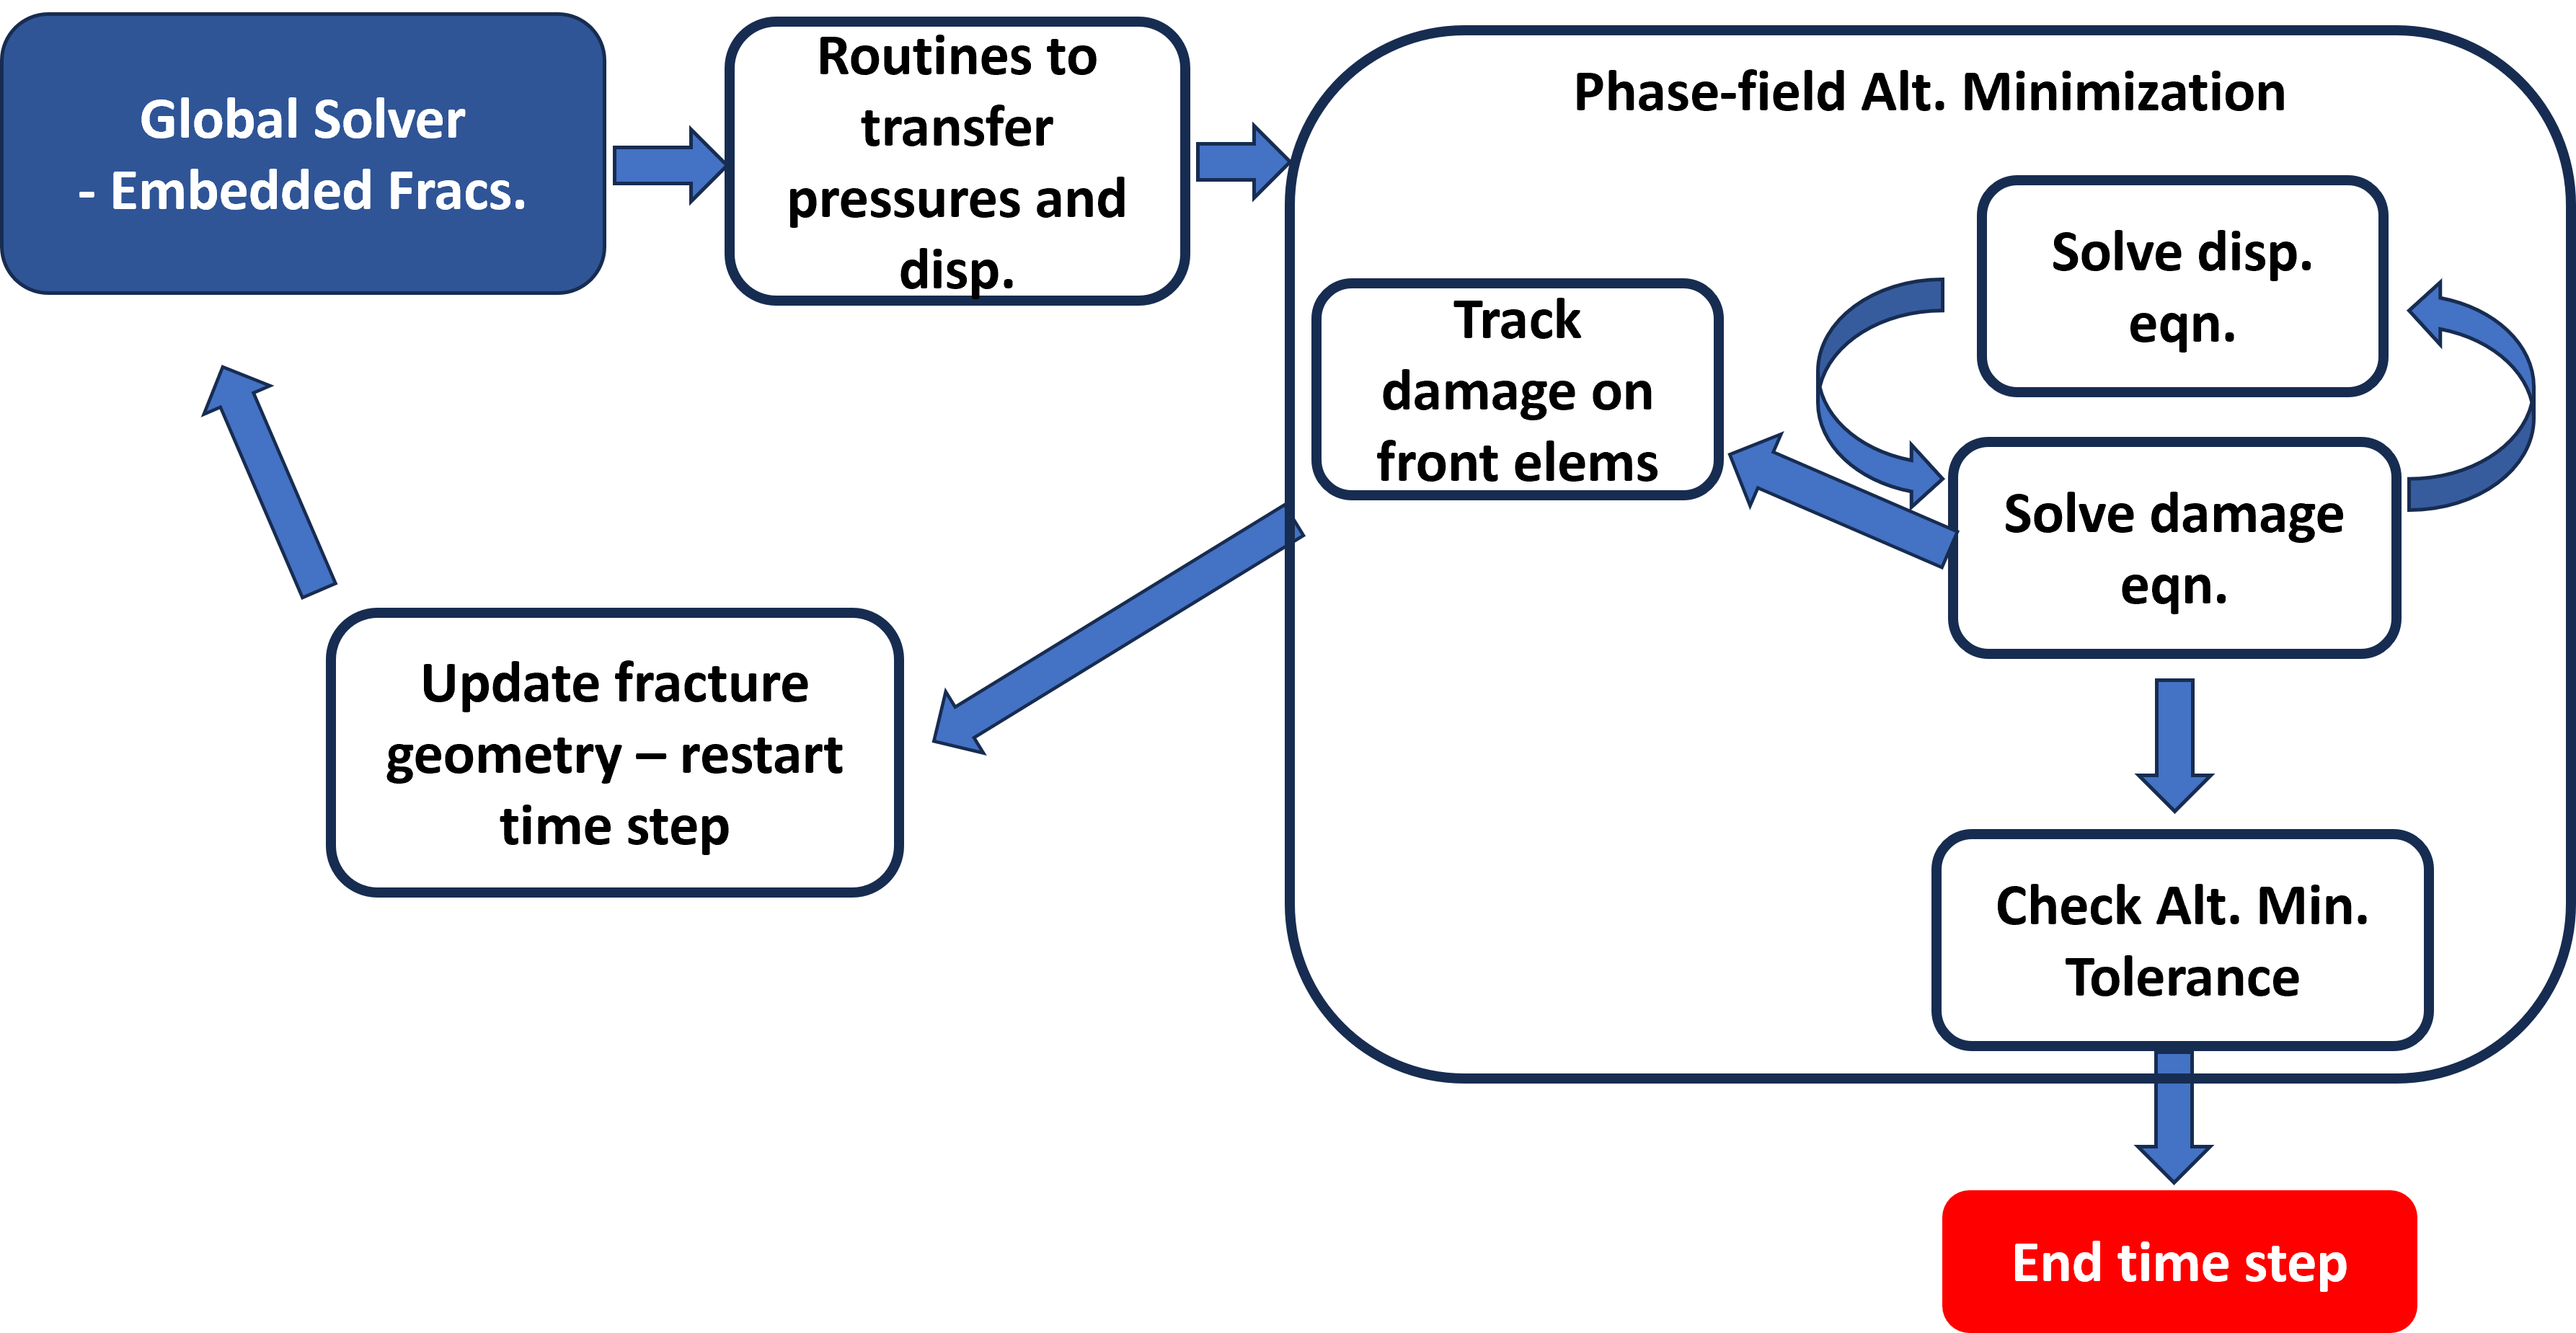
\includegraphics[width=\linewidth]{Chapter4/figures/planar3D_algorithm.png}
    \caption{Multi-resolution solution algorithm.}
    \label{fig:MR_planar_algo}
\end{figure}

A high-level description of the propagation algorithm for planar fractures in 3D is shown in Figure \ref{fig:MR_planar_algo}. It summarizes each of the steps involved in the solution procedure for a single time-setp. The process begins with the solution of the global problem (i.e, the box colored in blue in \ref{fig:MR_planar_algo}). As pointed out in chapter \ref{section: Chapter3}, the algorithm is agnostic with respect to the numerical methods employed. The approximate fields for pressure and displacements are then transfered to the local problem, as explained in the steps (3) and (4) of Algorithm \ref{fig:solution_algorithm}.

In the 2D algorithm, one would now move to the solution of the local problem with an alternate minimization approach and only then check for fracture propagation. In the proposed 3D algorithm, this is changed and a damage tracking function is launched in parallel with the damage solver. This function checks the amount of damage in the elements of the fracture front. Different measurements of damage can be employed, and they will likely depend on the discretization method employed. A simple one, which works well for planar fractures in structured grids is the volume of damage, which is defined as the total volume of subdiscretization' elements with damage above a threshold (usually around 0.9). This approach is effective since, for planar fractures aligned with structured grids, the fracture area on each element can be predicted beforehand. This simpliefied criteria is used in the example problems that will be shown next. For more general discretization types, a more robust approach is to identify the maximum damage level on each of the element faces. 

MENTION THAT PROPAGATION CRITERIA IS DISCRETIZATION DEPENDENT

If any of the front elements is identified as being cracked (i.e, the level of damage on it is very high), the alternate minimization iterations are halted. The geometry of the discrete fracture in the global is then updated. This update consists of the addition of a planar cut in this cracked element, followed by an advance in the fracture front. This sequence of steps is refered as \textit{propagation criteria}.

If multiple front elements are cracked, this process is done for all of them. The current time-step is then re-launched. Convergence is achieved when the alternate minization procedure reaches a tolerance without triggering the propagation criteria. When that happens, an equilibrium state is obtained and the time-step can be advanced.

\subsection{Fracture front construction}

The fracture front plays an important role in the propagation criteria. It greatly reduces the computational expense associated with the inspection of damage in the global elements while also serving to indicate a reference position to place the subdomains as the crack advances. It's construction happens during the initial discretization of the fracture in the global domain. One goes over all fractured elements and among its neighbors, adding those that share a fractured face but are not fracture to the front. This step is repeated every time the global fracture geometry is updated (i.e new fracture cells are inserted). Figure \ref{fig:crack_front} shows the fracture front for an initial discretization (and fairly coarse) of a penny shaped fractured.
Figure \ref{fig:crack_prop_steps} shows the sequence of steps involved in the fracture propagation process, including the update of the fracture front.

\begin{figure}[h]
    \centering
    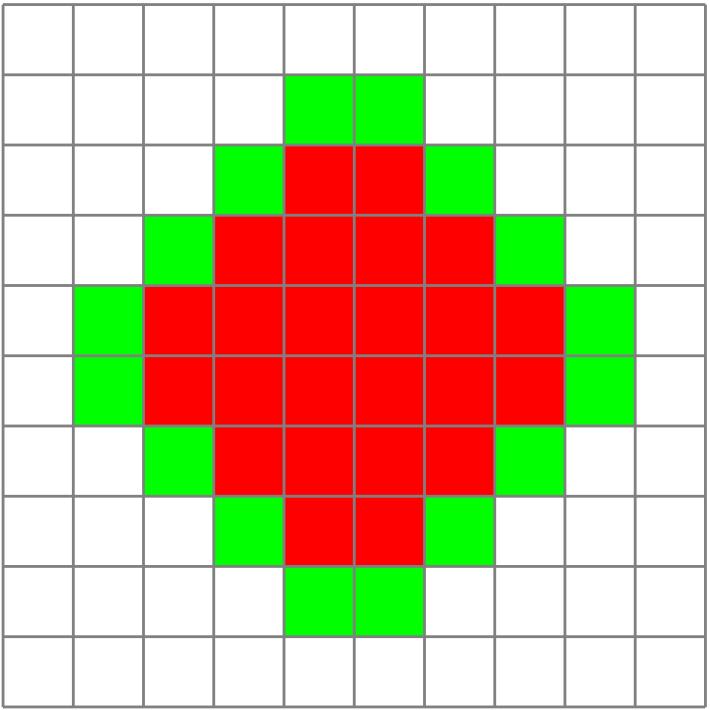
\includegraphics[width=0.4\linewidth]{Chapter4/figures/front_penny.png}
    \caption{Front elements shown in green. Red elements represent discretized fracture.}
    \label{fig:crack_front}
\end{figure}

\begin{figure}[h]
    \begin{subfigure}{\textwidth}
        \hspace*{1.85cm}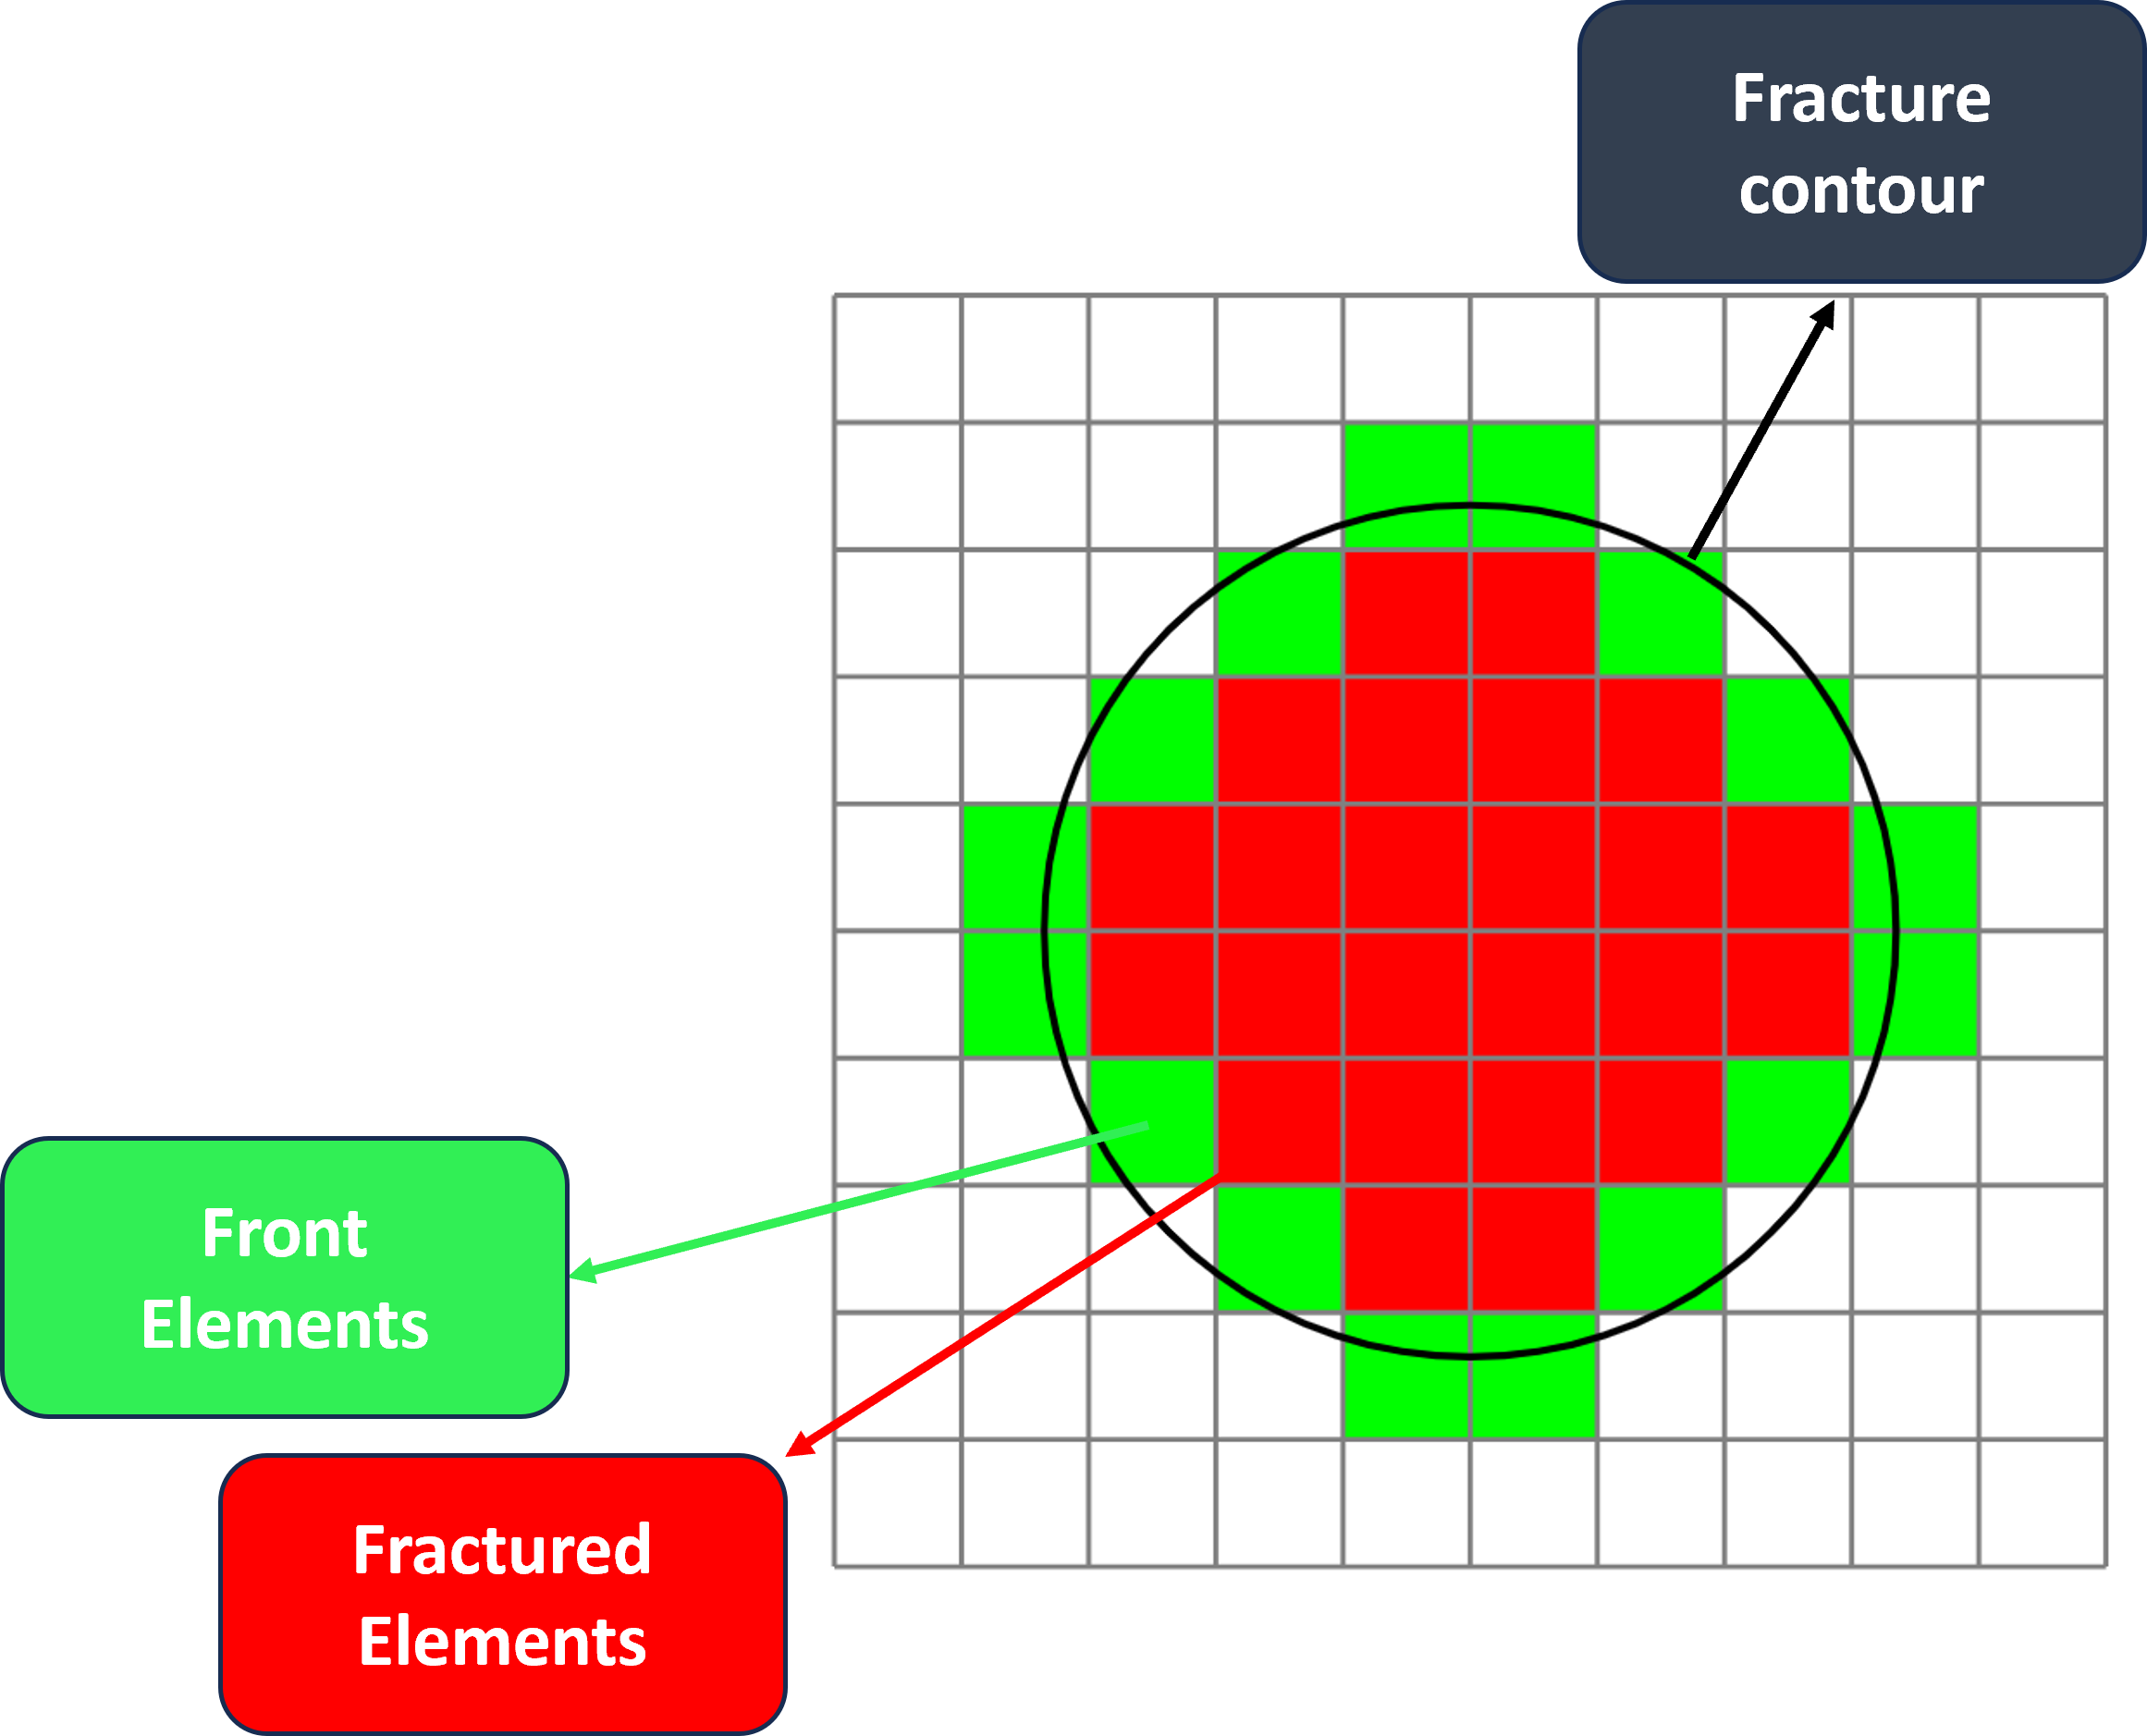
\includegraphics[width=0.55\linewidth]{Chapter4/figures/penny_with_descriptions.png}
        \caption{Initial state.}
        \label{fig:lorem1}
    \end{subfigure}

    \begin{subfigure}{\textwidth}    
        \hspace*{2.35cm}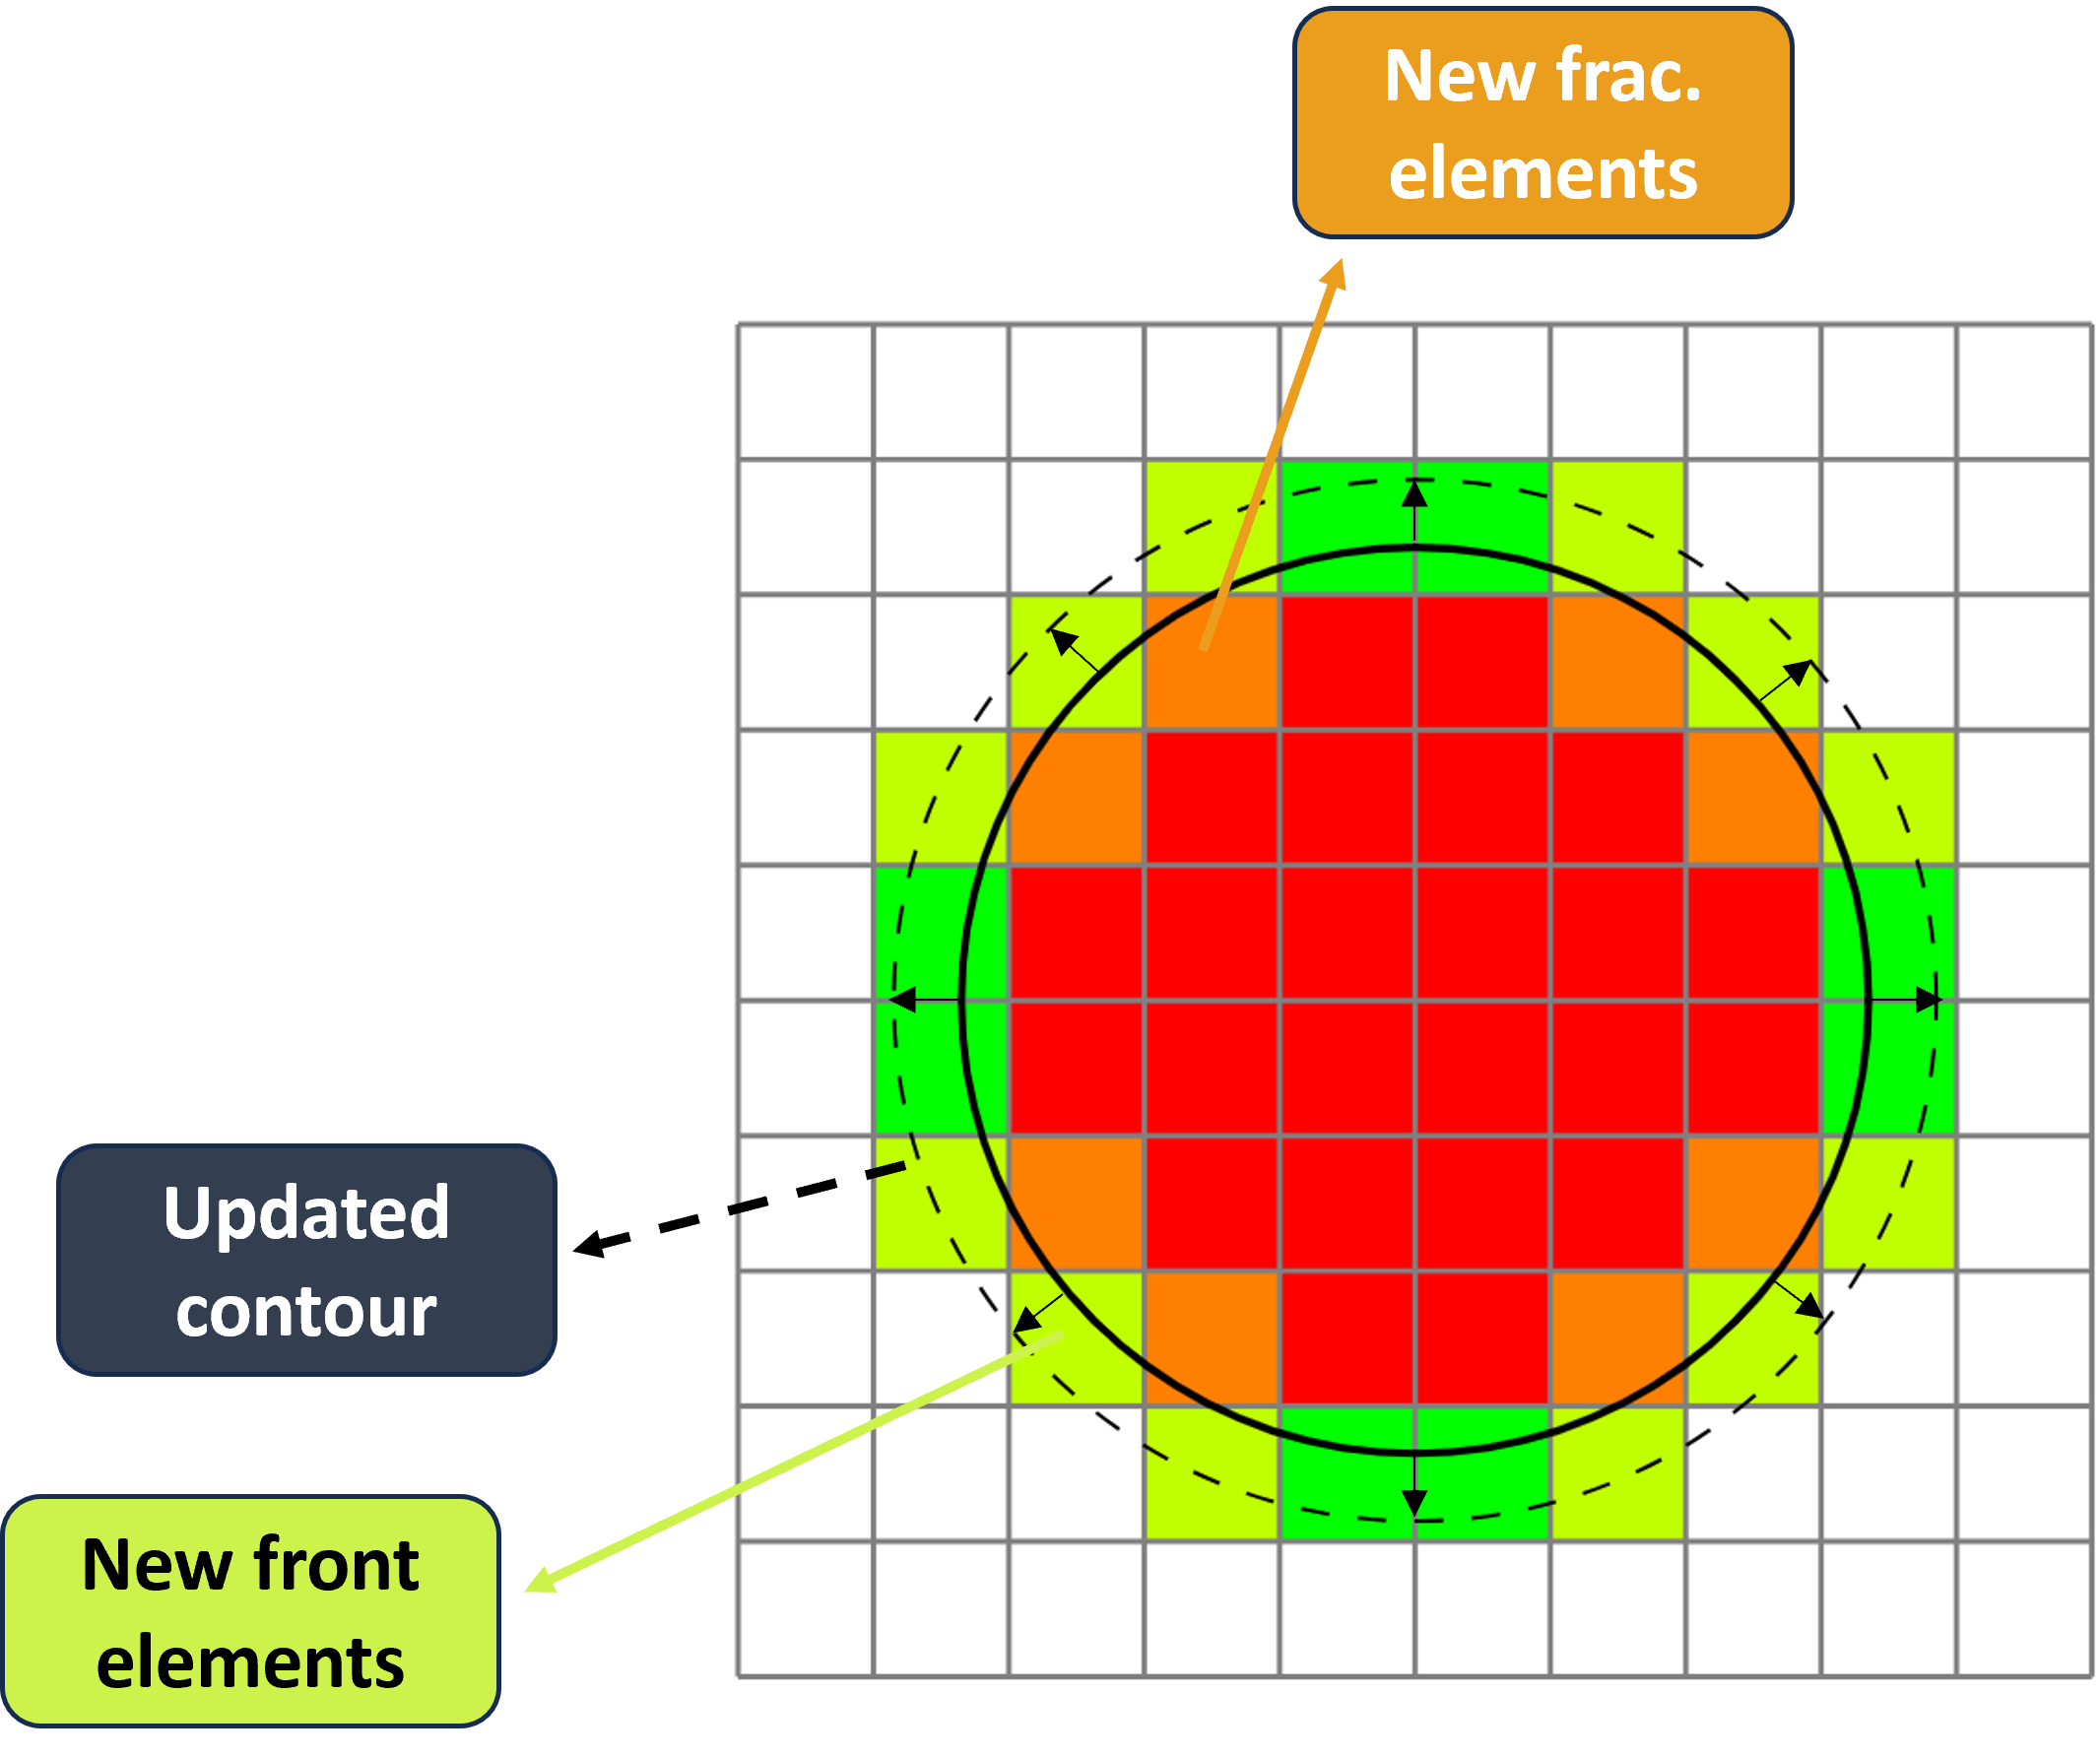
\includegraphics[width=0.51\linewidth]{Chapter4/figures/larger_penny_with_descriptions.png}
        \caption{Damage advanced.}
        \label{fig:lorem2}
    \end{subfigure}
    
    \begin{subfigure}{\textwidth}
        \centering
        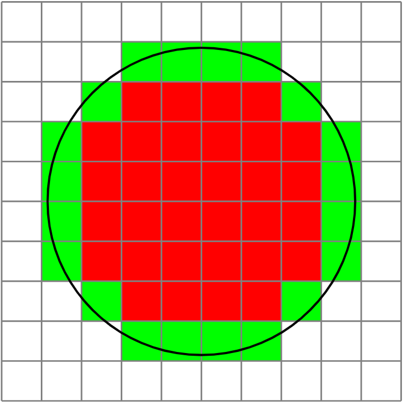
\includegraphics[width=0.33\linewidth]{Chapter4/figures/larger_penny.png}
        \caption{Updated configuration.}
        \label{fig:lorem3}
    \end{subfigure}
    \caption{Schematic of propagation steps.}
    \label{fig:crack_prop_steps}
\end{figure}

\subsection{Tracking damage in the fracture front elements}

The process of tracking the damage in the front elements also deserves a more detailed explanation. In the set of preliminary results shown next, a simplified method suitable for planar cracks in structured grids is used. It consists of first computing the cross sectional area of the element along the fracture plane. For example, for a fracture whose normal is in the x direction, one gets $H_yH_z$.\footnote{Assume that the global element has dimensions $H_x, H_y$ and $H_z$ whereas the local one has $h_x, h_y$ and $h_z$.} This is only possible when the structured grid is aligned with the fracture (either in $x, y$ or $z$).

Then, assuming that the fully damaged region of a phase-field fracture consists of a single element \footnote{this is not so obvious} across the band width, one expects the fully cracked region to have a volume of $h_xH_yH_z$. A simple criteria then consists of measuring the volume of local elements that have reached an average damage beyond a threshold close to 1 (In the examples shown next, this threshold was set to 0.9). A global element is then considered fractured if this volume reaches $h_xH_yH_z$.

This method contains multiple limitations, such as the need for planar fractures aligned with a structured grid and also the hypothesis that the damage band has a single fully degraded element along its width. An alternative method to circunvent these issues inspired by \cite{muixi2021combined} consists of evaluating the damage field in the edges of an element. It assumes that a fractured element has at least three fractured faces and that a fractured face is cut on two of its edges.

For each global element in the crack front, the damage field, computed in the local mesh, is inspected on every edge. If damage above a threshold (typically 0.9 or 0.95) is identified in a given edge, that edge is considered cut. If any face contains two cut edges, it is marked as cut. An element is then marked as fracture when at least three of its faces are cut.

This criteria circunvents some of the limitations of the simpliefied one, removing the need for structured grids. It is also applicable to nonplanar fractures as well. However, it is not perfectly robust and certain relative configurations between the damage field and the global element in the front can lead to unexpected results. This will be shown in Section \ref{section: Chapter4/nonplanar} that discusses the case of nonplanar fractures.


% \begin{figure}[h]
%     \centering
%     \begin{subfigure}{.45\textwidth}
%         \centering
%         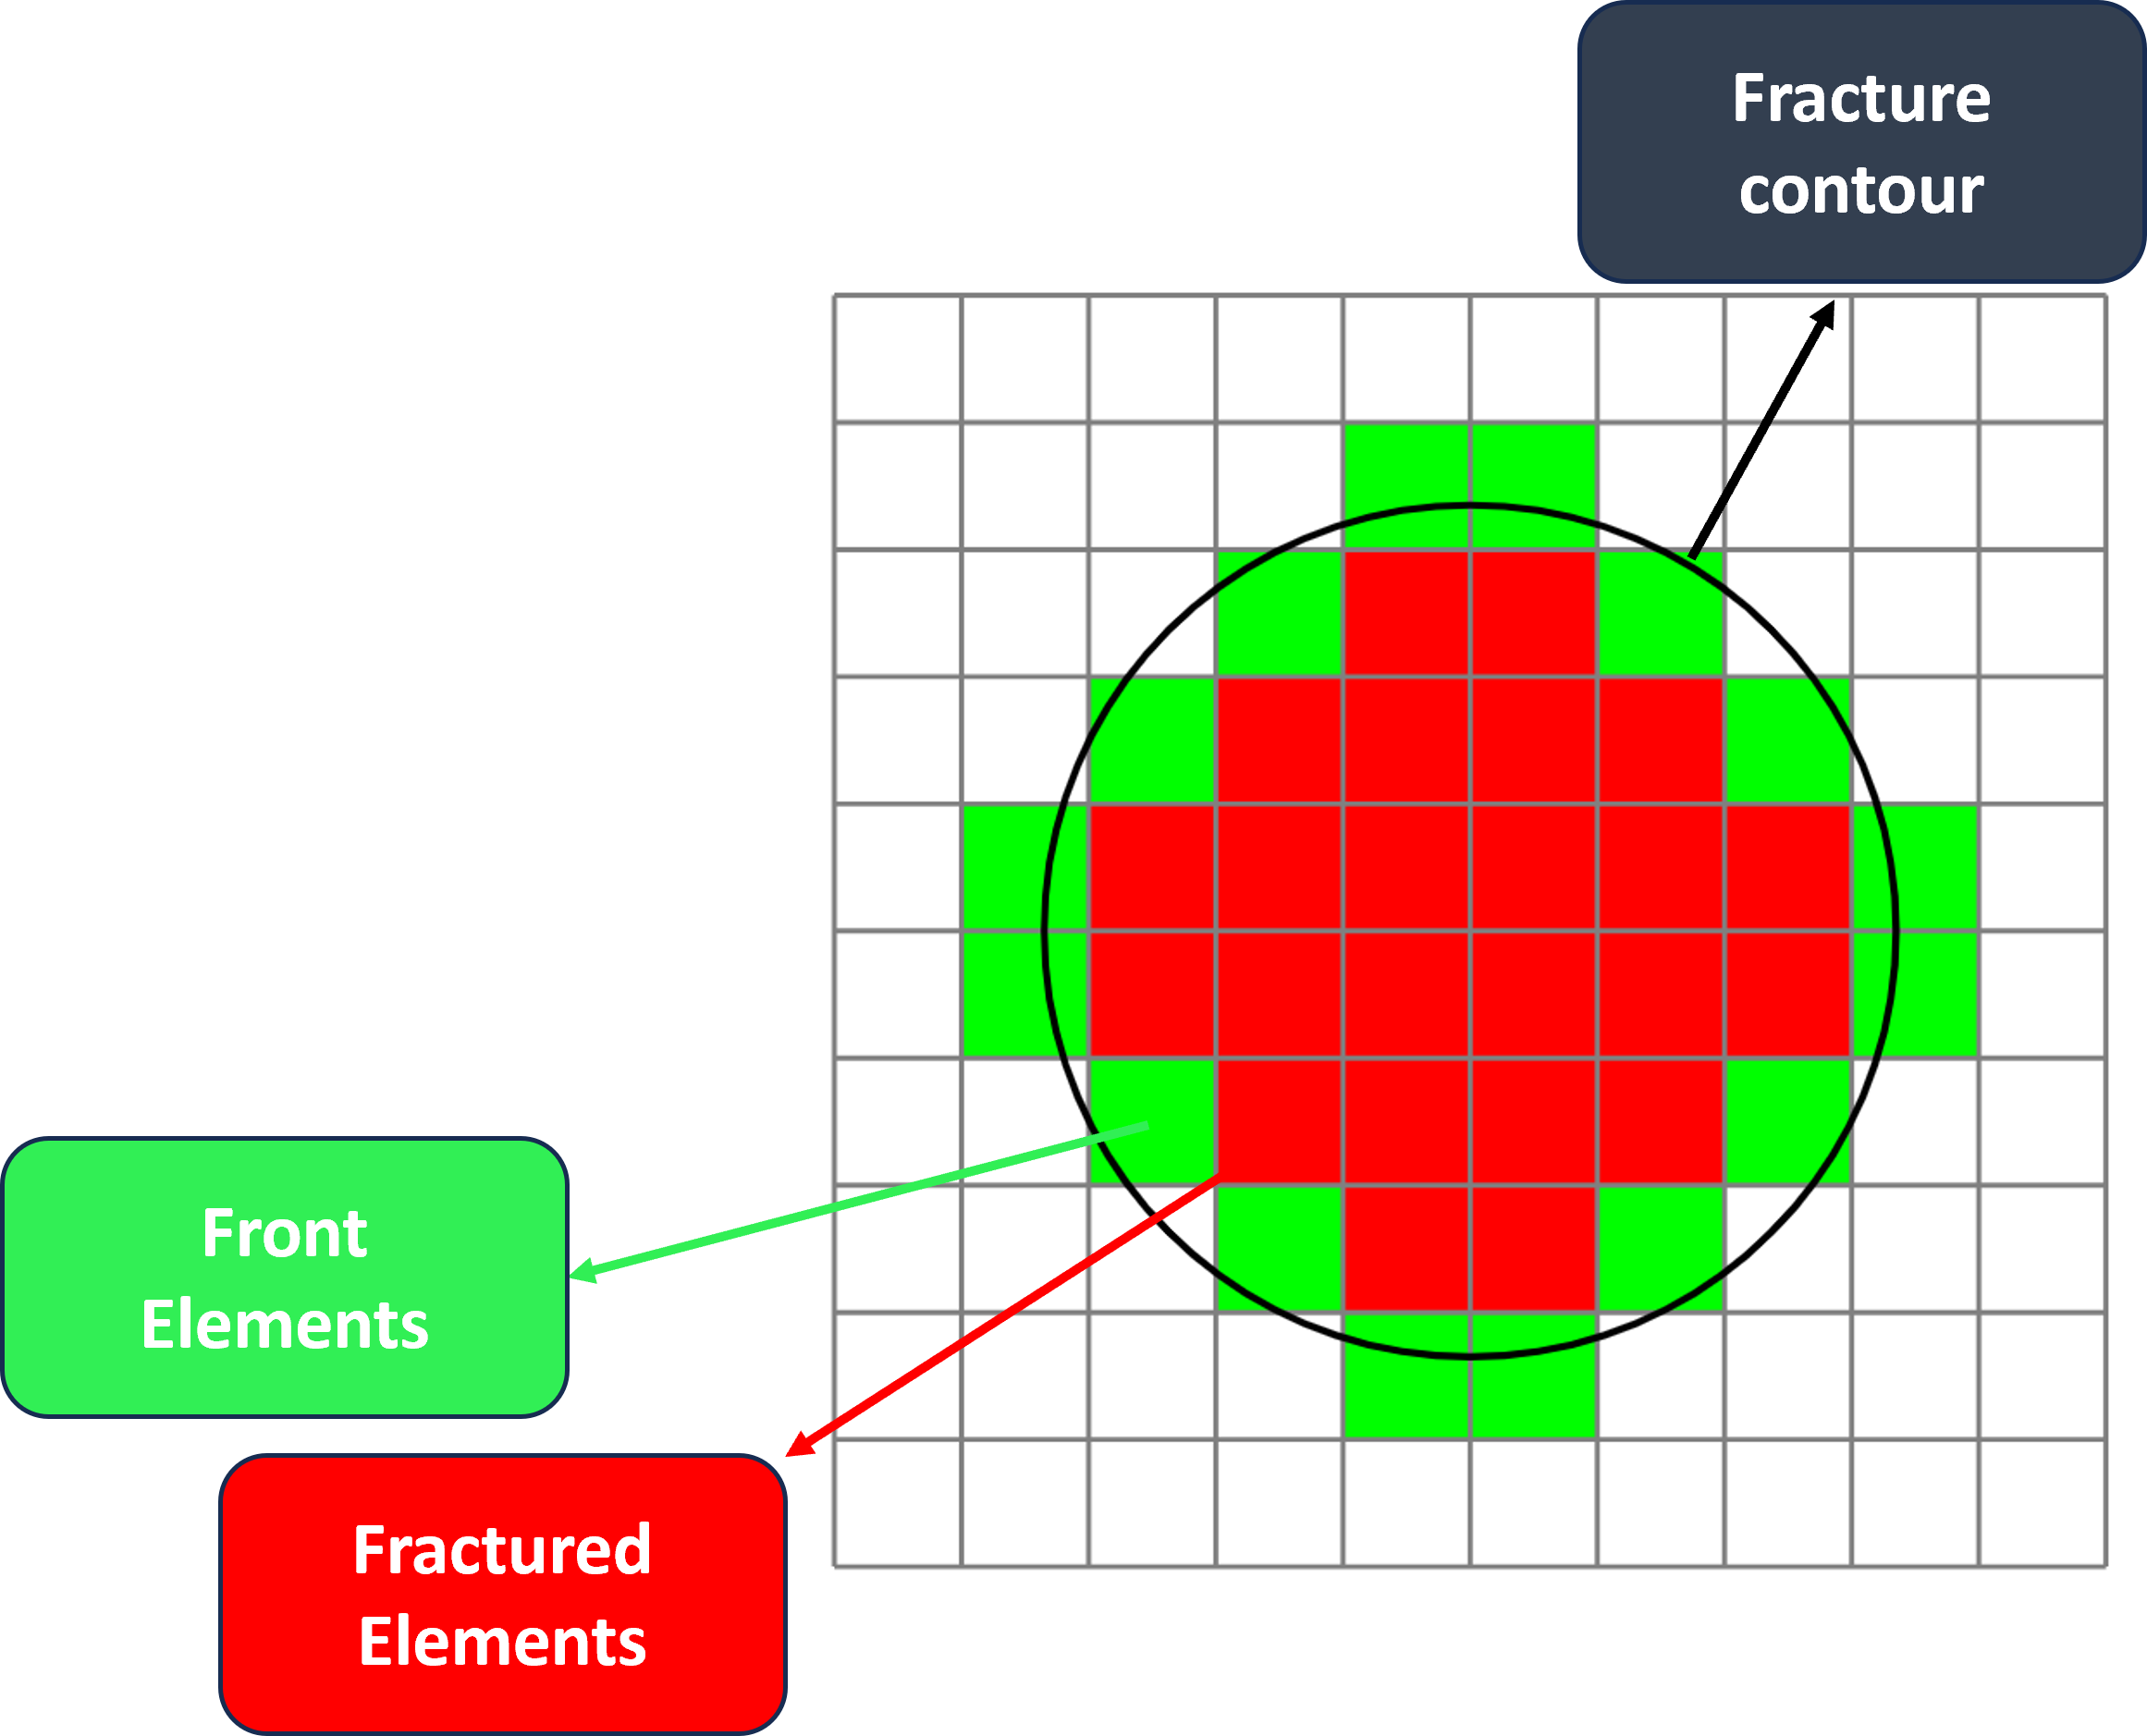
\includegraphics[width=\linewidth]{Chapter4/figures/penny_with_descriptions.png}
%         \caption{Multi-resolution solution algorithm.}
%         \label{fig:lorem1}
%     \end{subfigure}%
%     \begin{subfigure}{.45\textwidth}
%         \centering
%         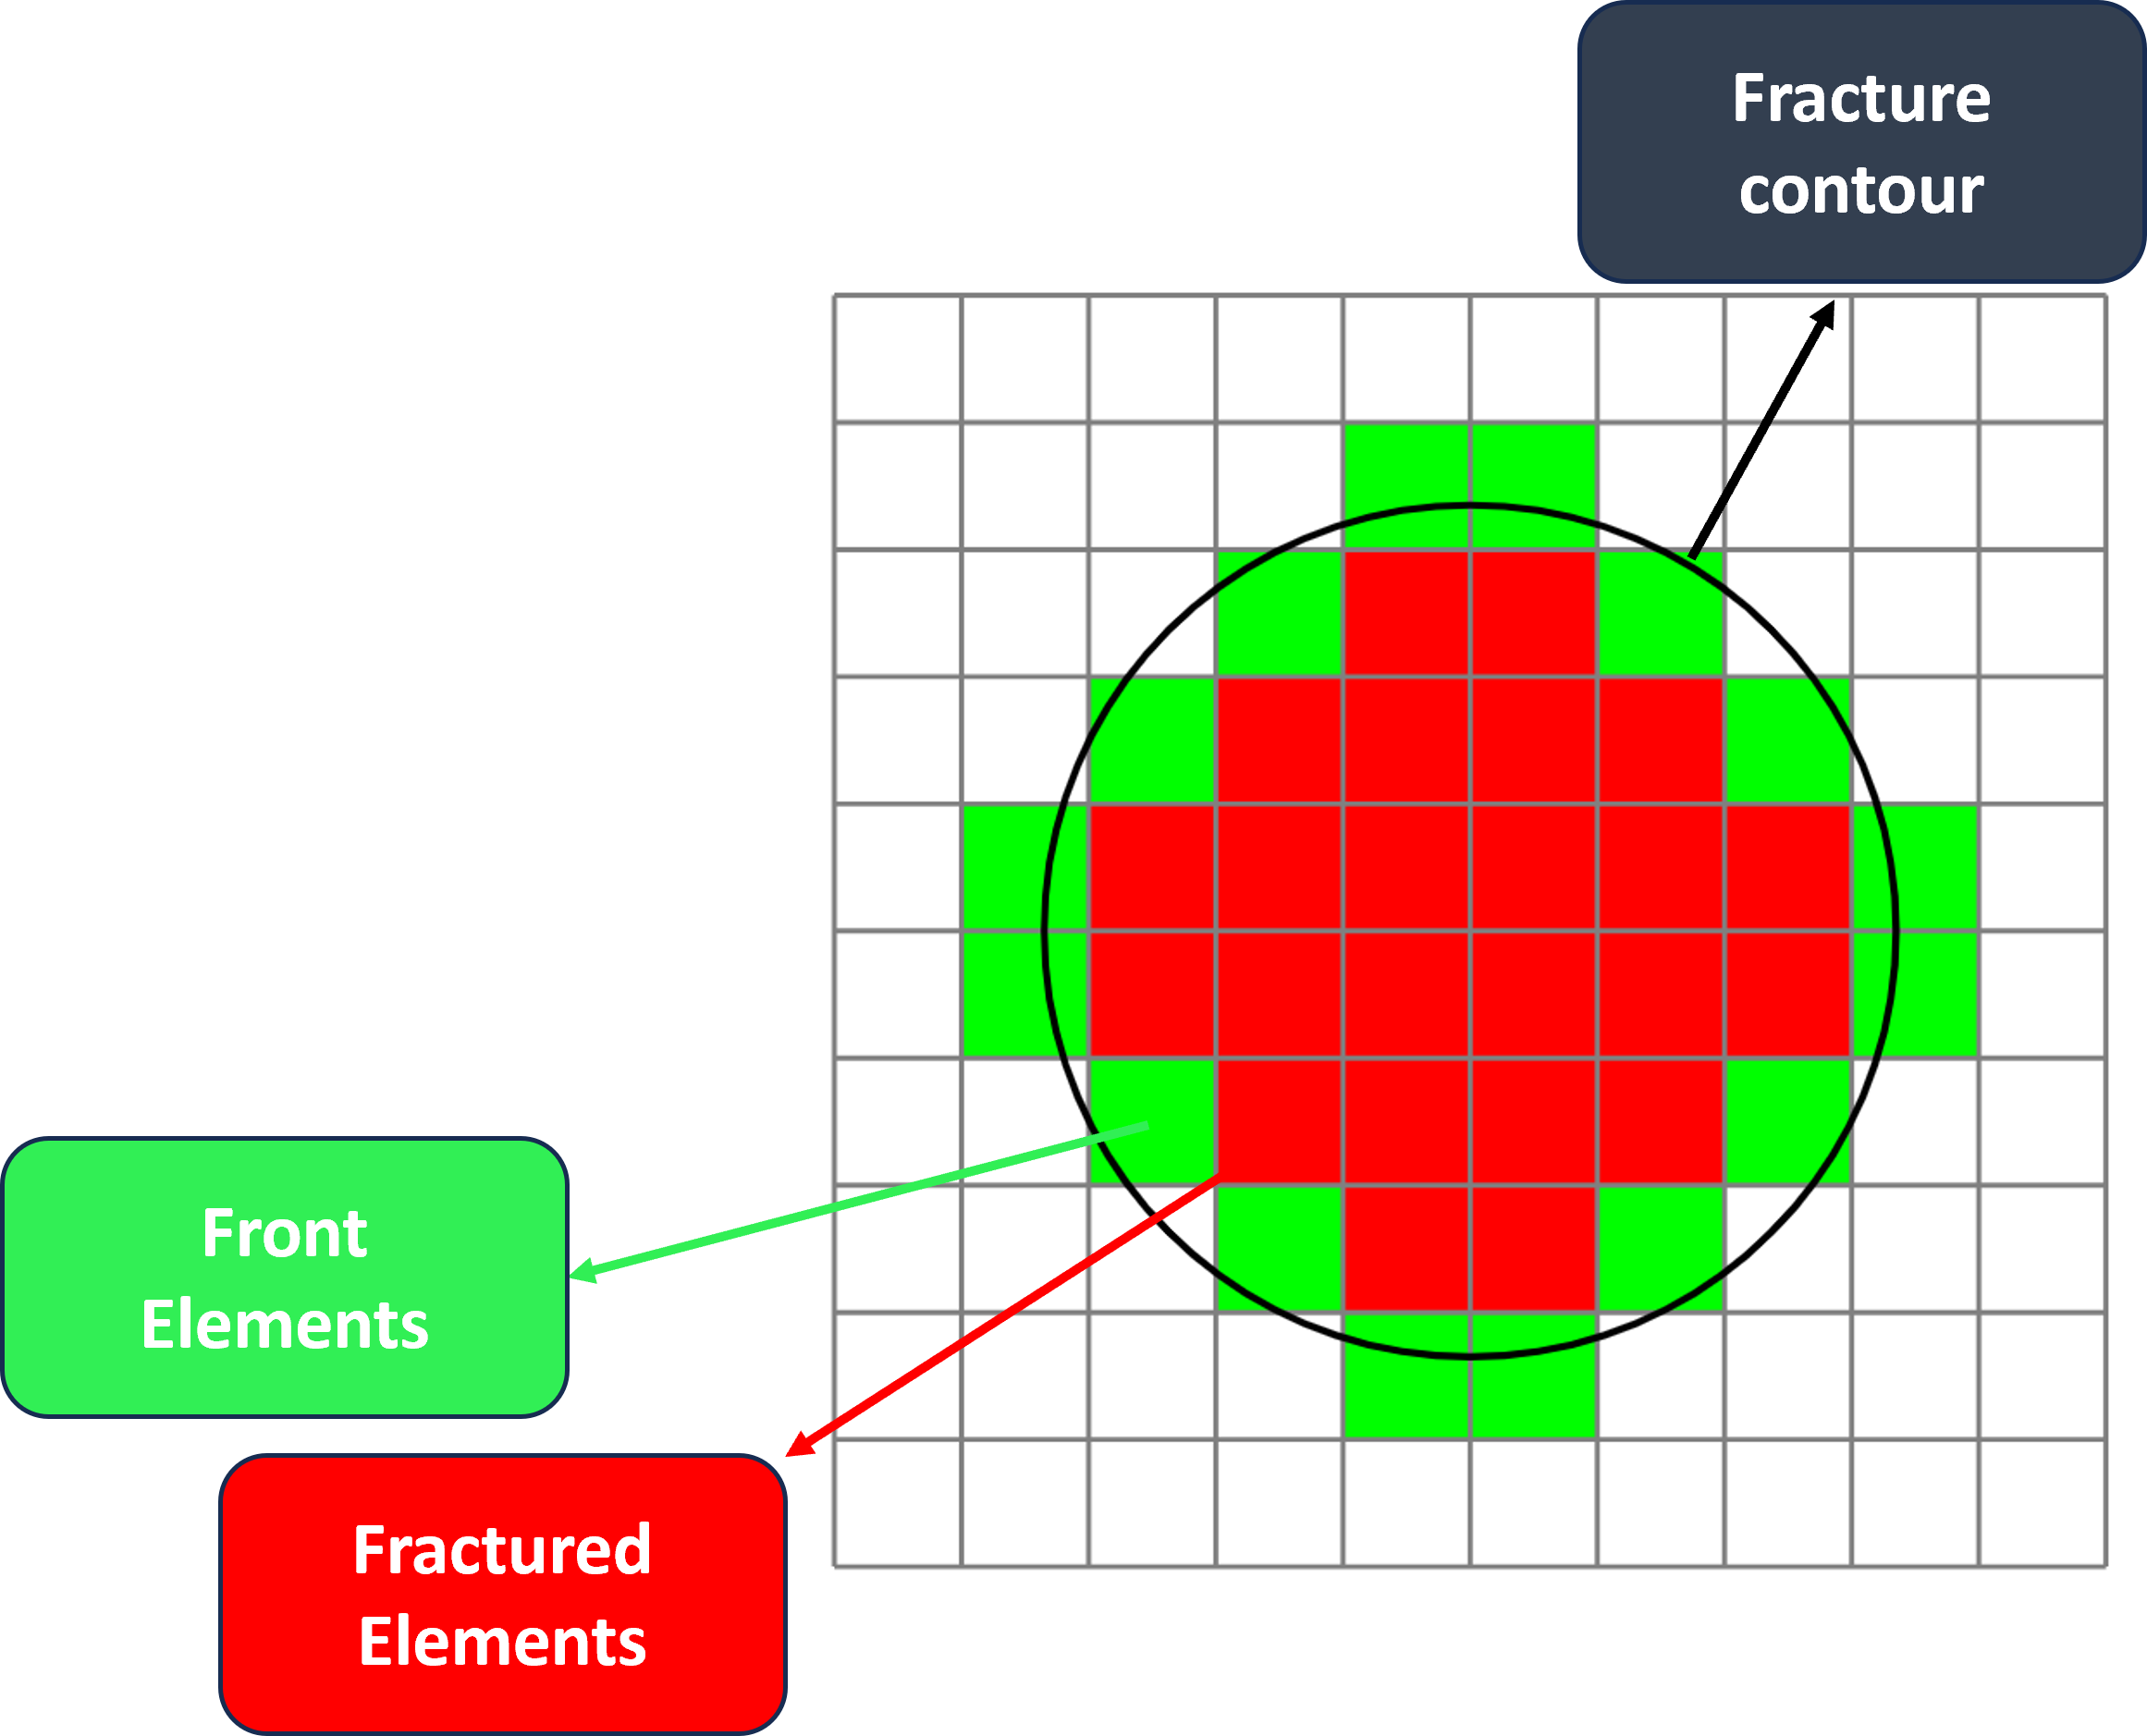
\includegraphics[width=\linewidth]{Chapter4/figures/penny_with_descriptions.png}
%         \caption{Multi-resolution solution algorithm.}
%         \label{fig:lorem2}
%     \end{subfigure}%
    
%     \bigskip
%     \begin{subfigure}{.45\textwidth}
%         \centering
%         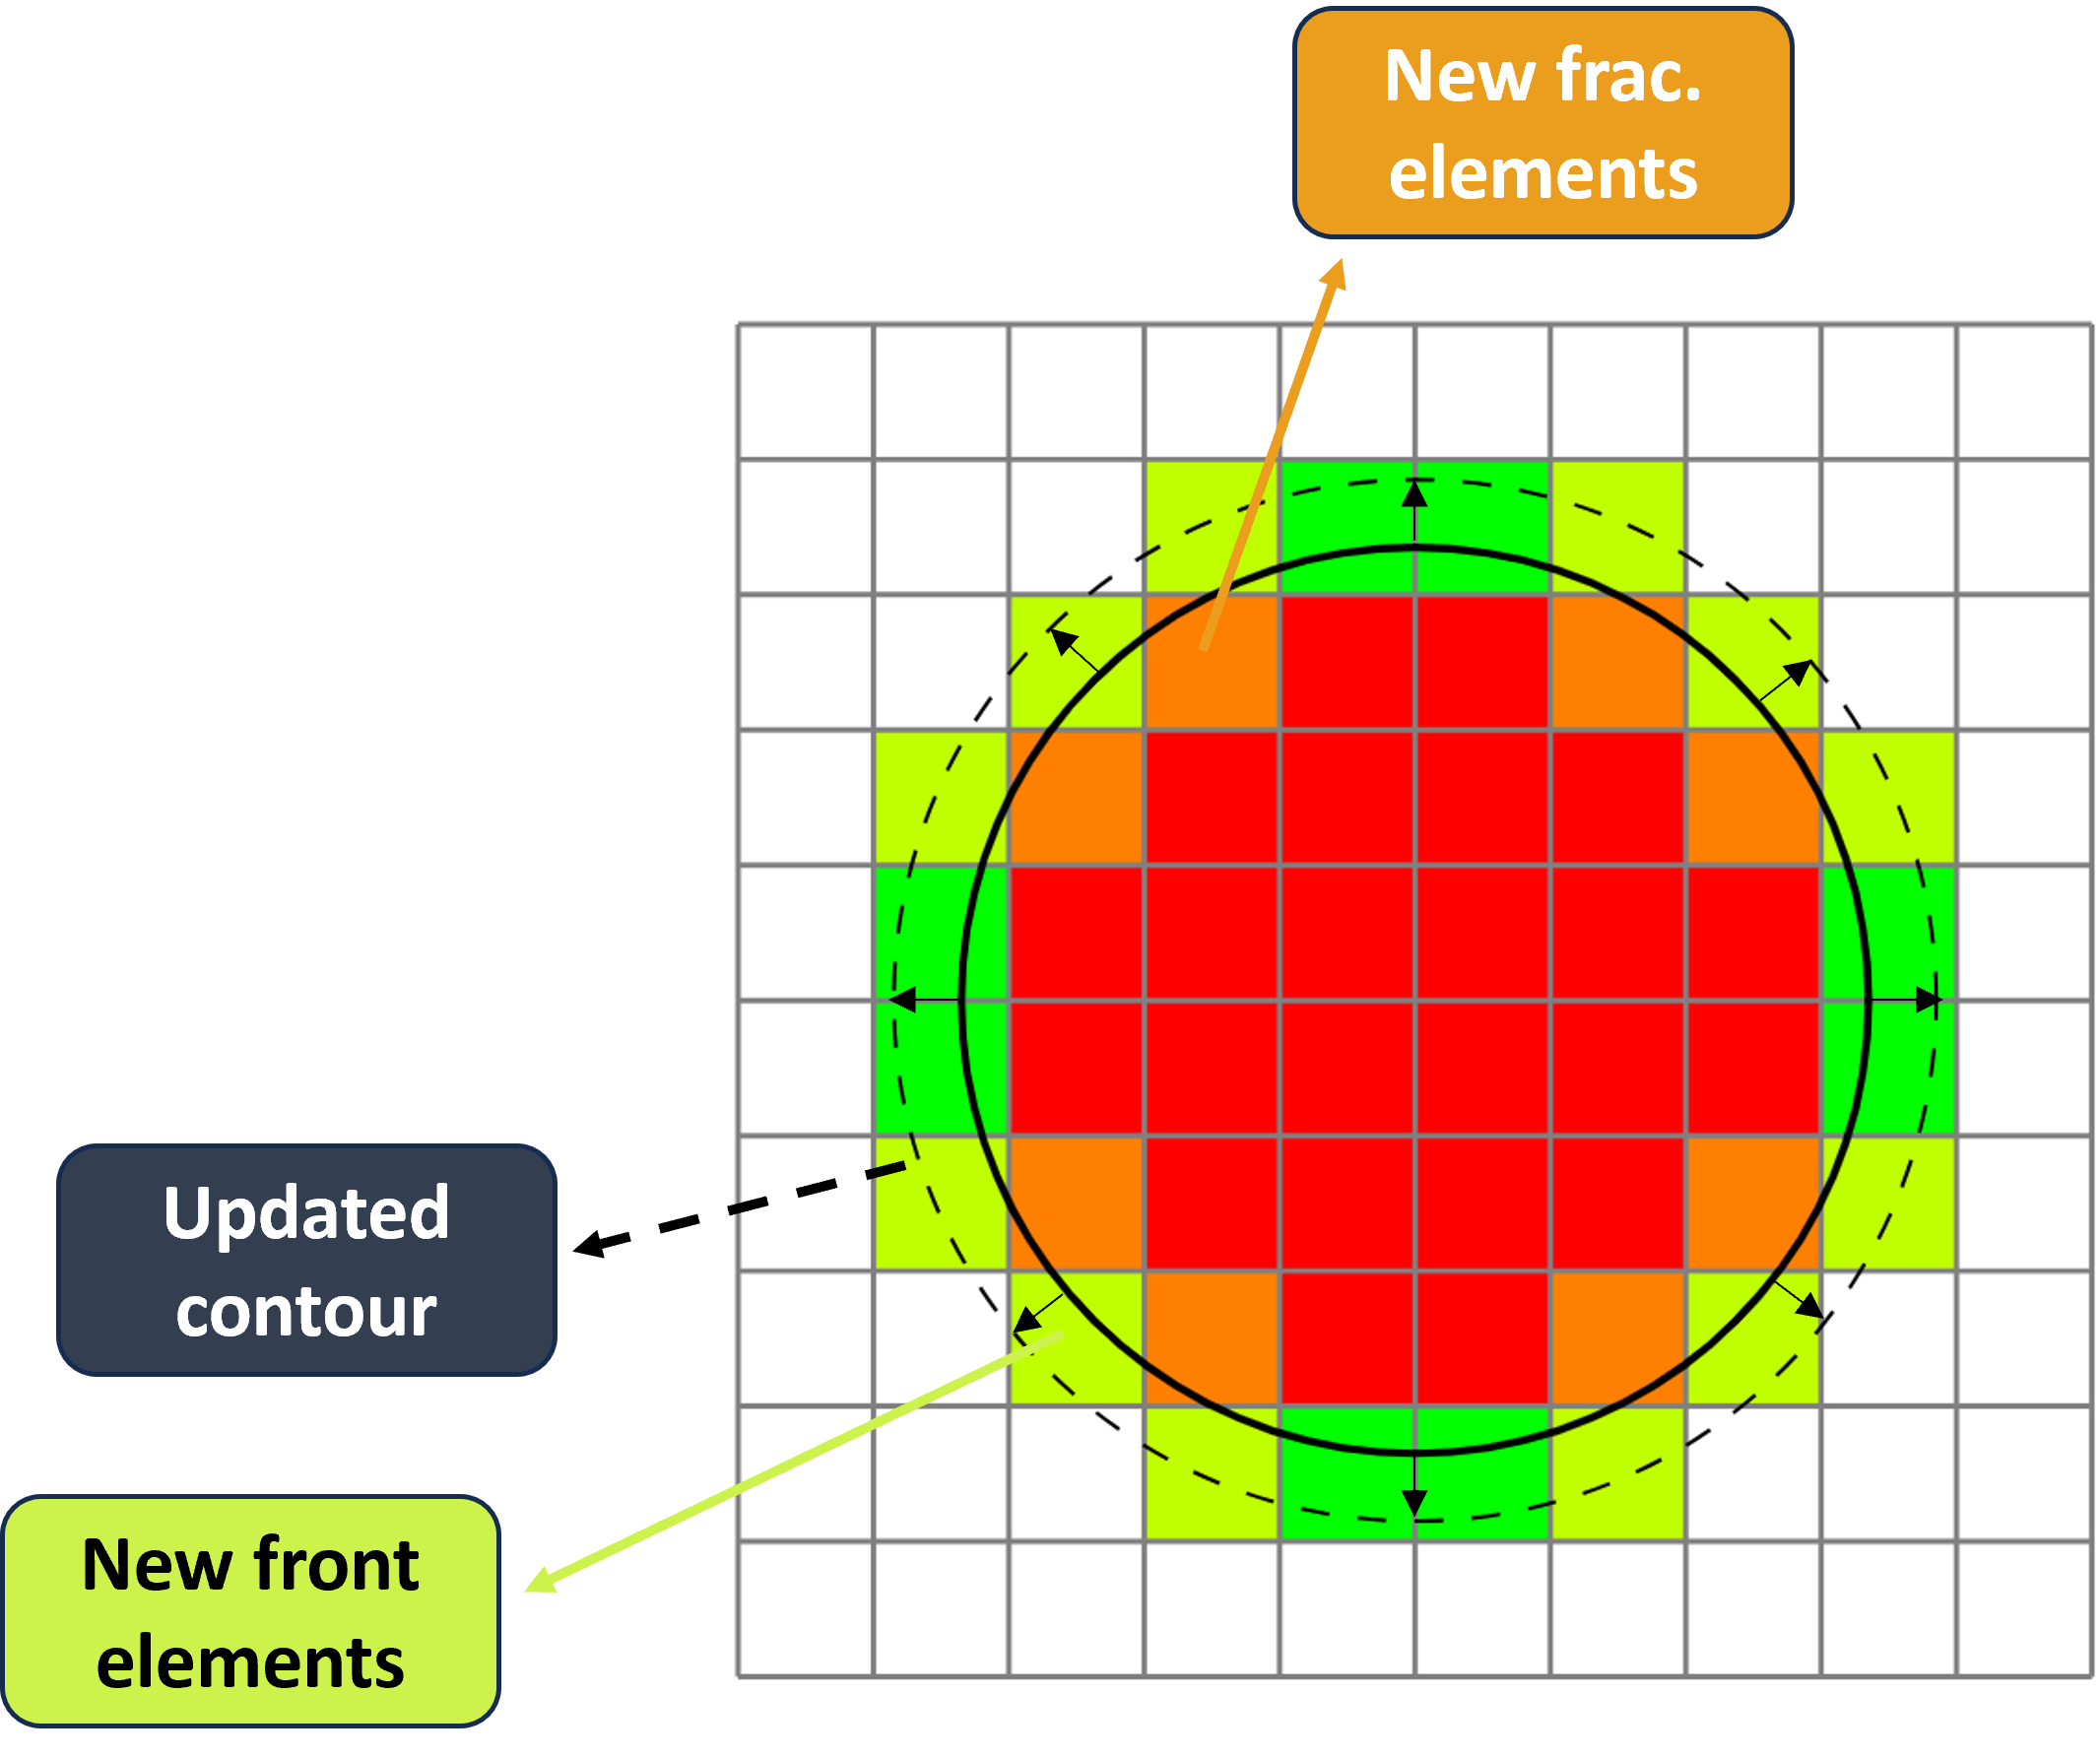
\includegraphics[width=\linewidth]{Chapter4/figures/larger_penny_with_descriptions.png}
%         \caption{Multi-resolution solution algorithm.}
%         \label{fig:lorem3}
%     \end{subfigure}
%     \begin{subfigure}{.45\textwidth}
%         \centering
%         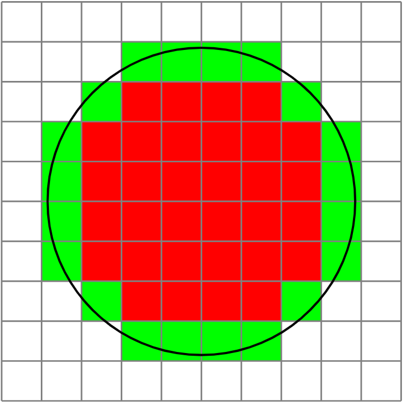
\includegraphics[width=0.65\linewidth]{Chapter4/figures/larger_penny.png}
%         \caption{Multi-resolution solution algorithm.}
%         \label{fig:lorem4}
%     \end{subfigure}
%       \caption{Schematic of propagation steps.}
% \end{figure}

% \begin{figure}[h]
%     \centering
%     \begin{subfigure}{\textwidth}
%         \centering
%         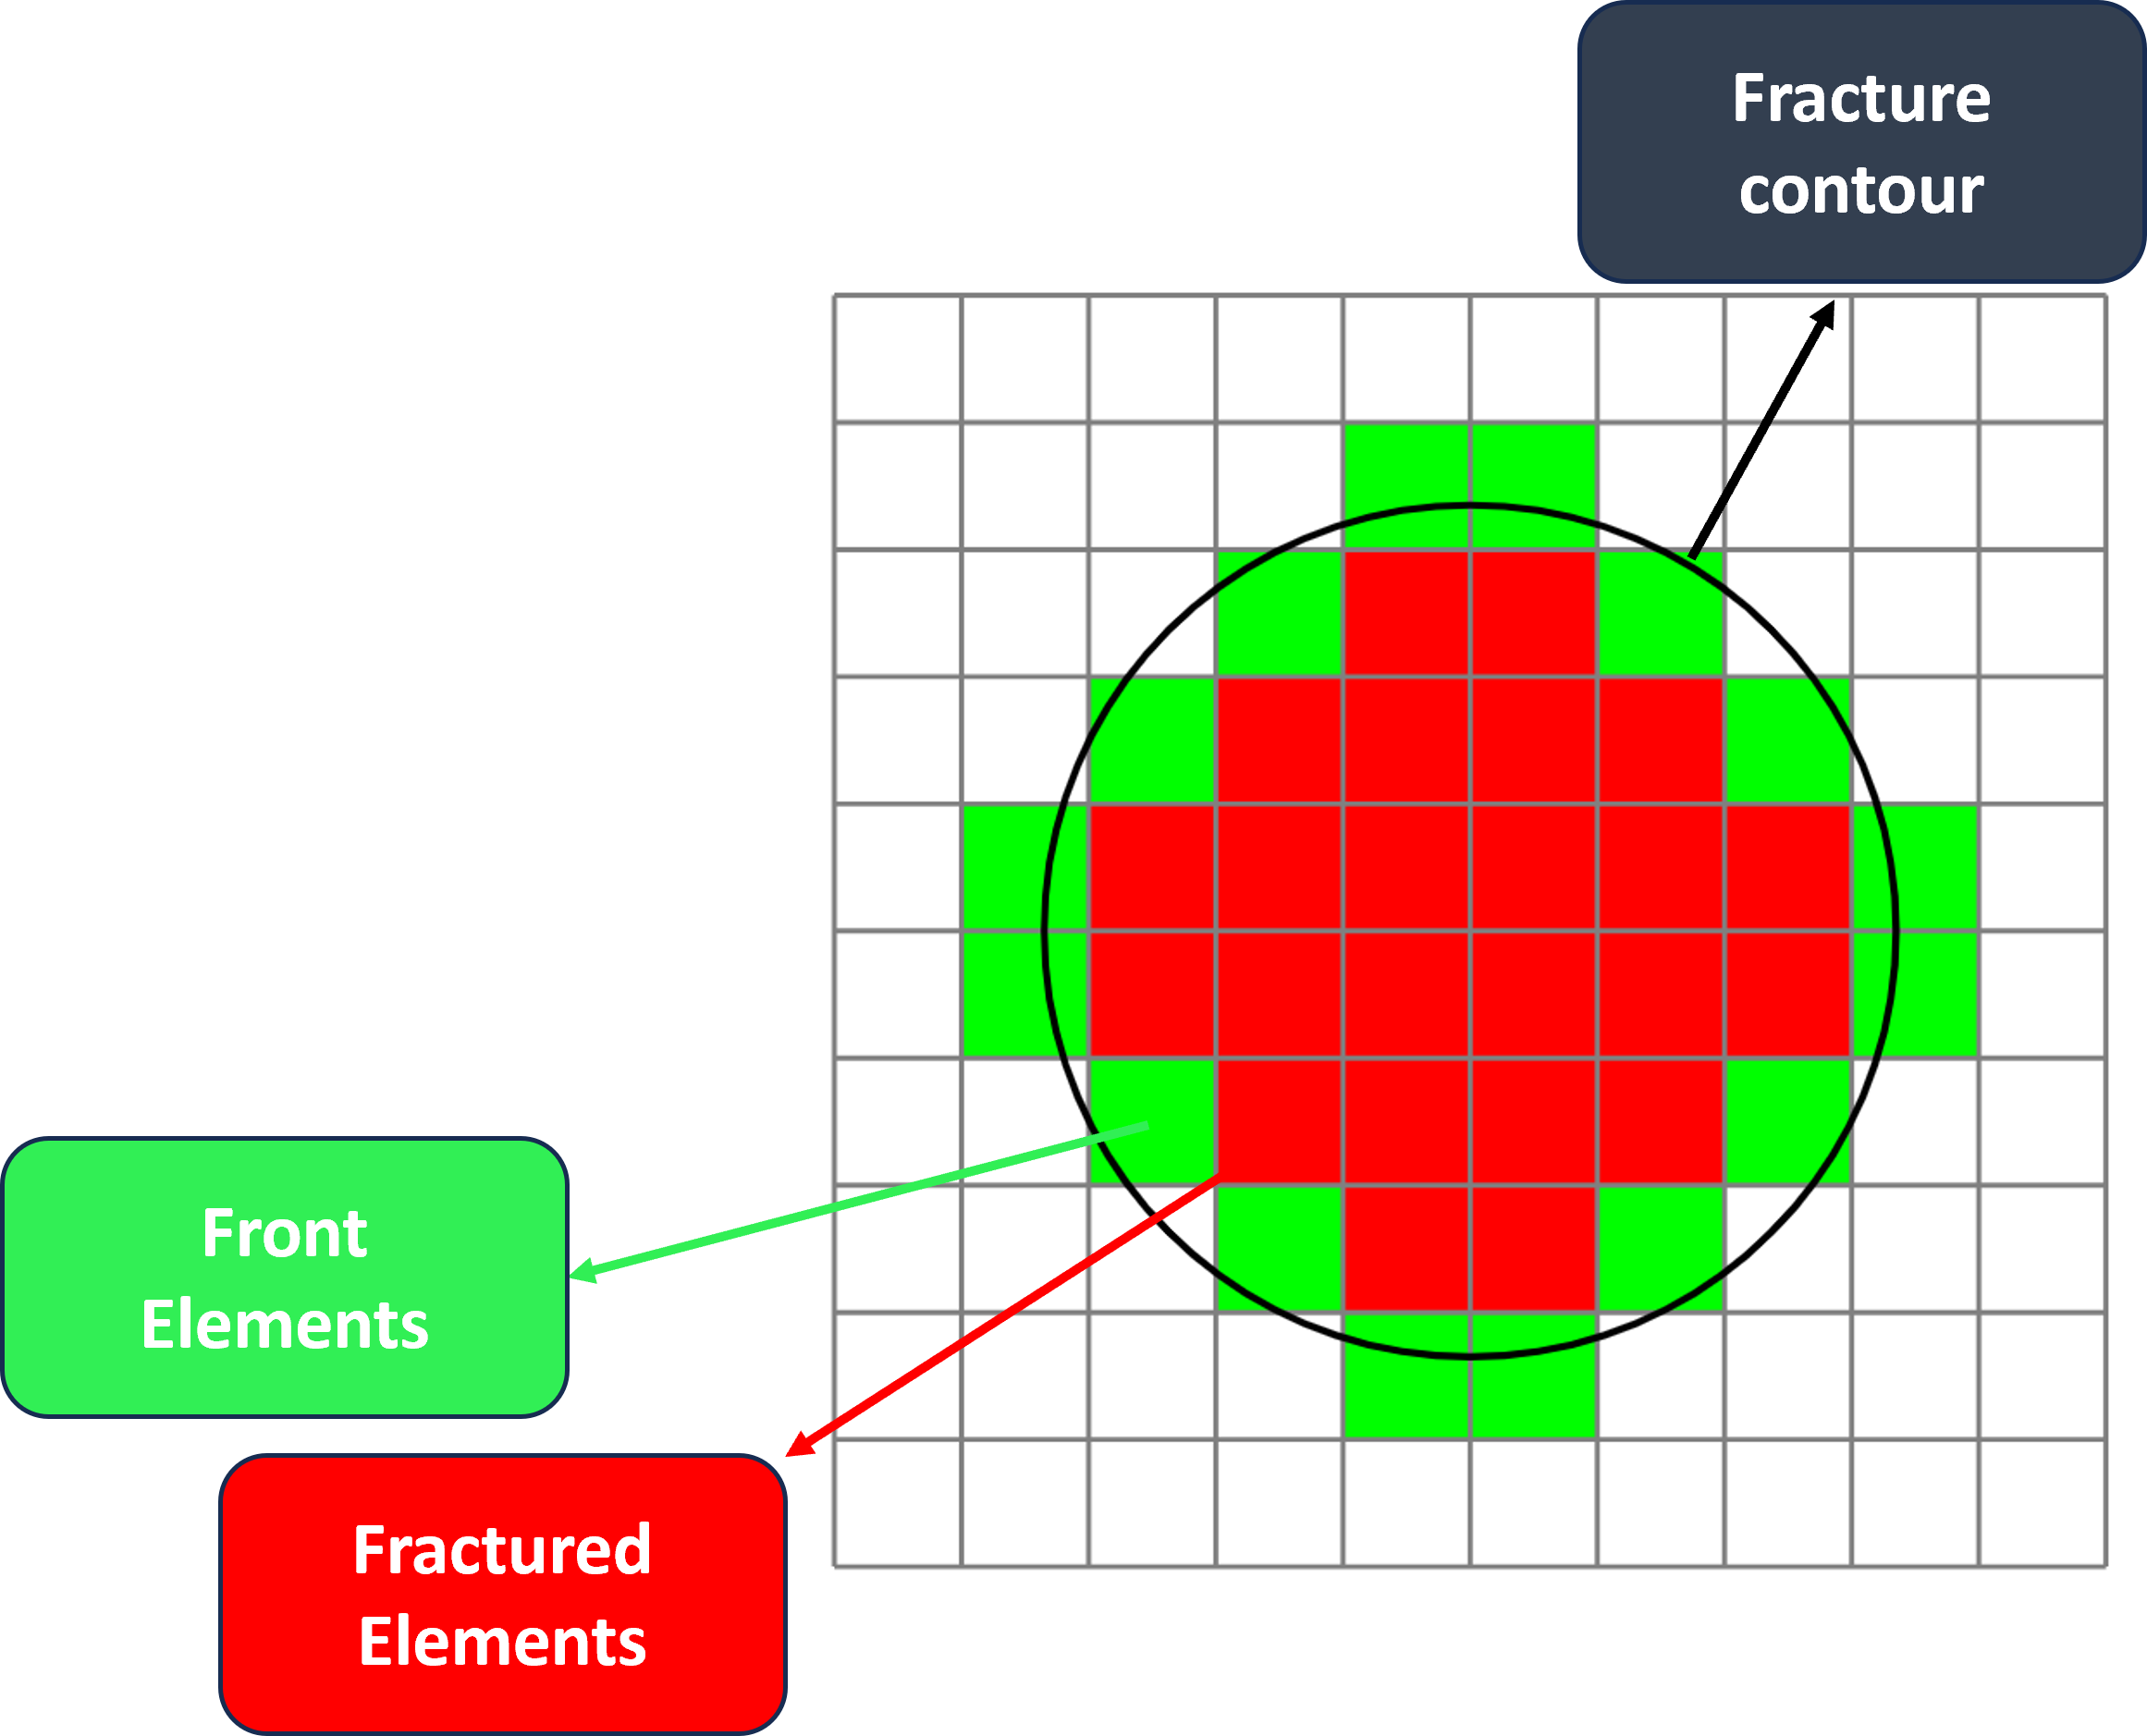
\includegraphics[width=\linewidth]{Chapter4/figures/penny_with_descriptions.png}
%         \caption{Multi-resolution solution algorithm.}
%         \label{fig:lorem1}
%     \end{subfigure}%
%     \bigskip
%     \begin{subfigure}{\textwidth}
%         \centering
%         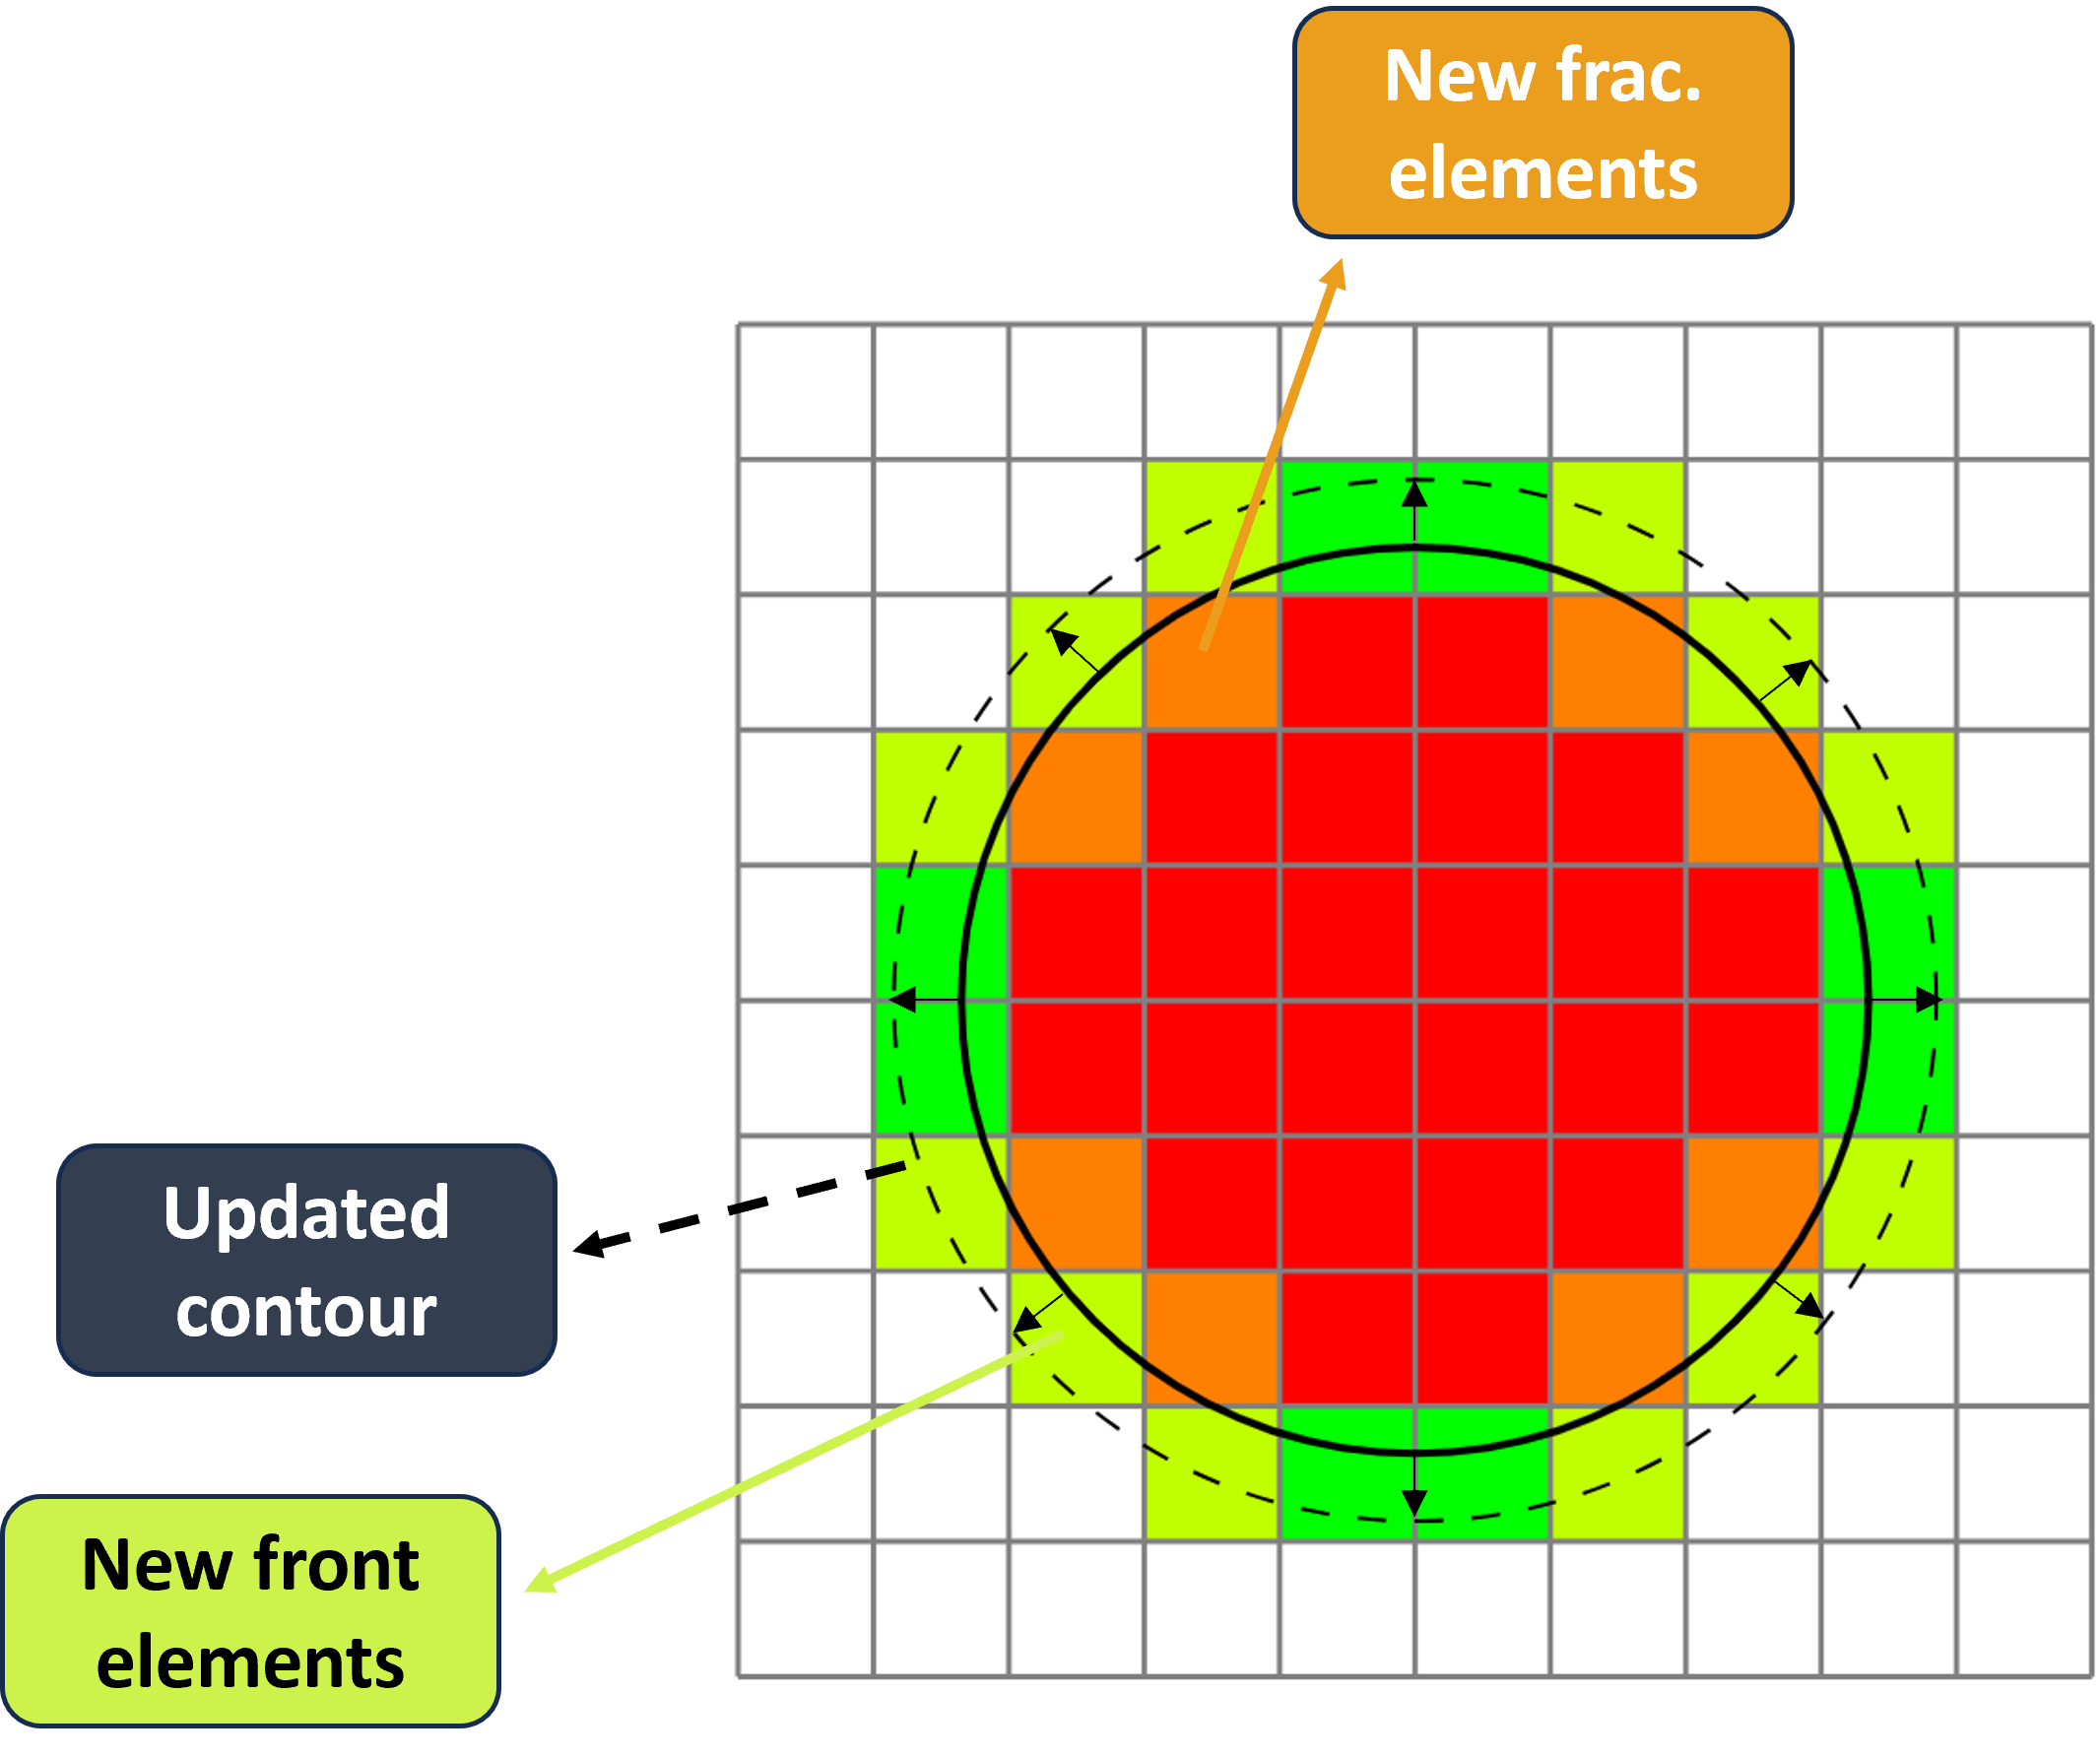
\includegraphics[width=\linewidth]{Chapter4/figures/larger_penny_with_descriptions.png}
%         \caption{Multi-resolution solution algorithm.}
%         \label{fig:lorem2}
%     \end{subfigure}
%     \bigskip
%     \begin{subfigure}{\textwidth}
%         \centering
%         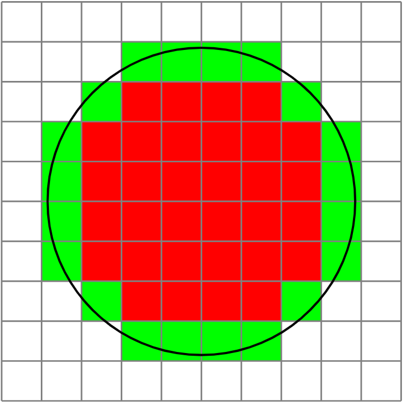
\includegraphics[width=0.65\linewidth]{Chapter4/figures/larger_penny.png}
%         \caption{Multi-resolution solution algorithm.}
%         \label{fig:lorem3}
%     \end{subfigure}
%     \caption{Schematic of propagation steps.}
% \end{figure}



